\subsection{Diseño del barrido}

Se corrieron los 15 kernels de dataset del catálogo (7 CPU, 8 GPU) diez
veces cada uno bajo la cadencia por defecto (150 corridas reales), para
poder calcular, sobre el mismo conjunto de datos, el CV\% de tiempo de
ejecución en función de cuántas de esas diez repeticiones se acumulan
($n=3,4,\ldots,10$) -- sin necesidad de una campaña nueva por cada valor de
$n$. Al procesar los resultados se encontró el mismo error de esta
herramienta de barrido ya descrito en la Sección~\ref{sec:interval-ns}
(\texttt{freq\_khz\_observed=None}); se corrigió de la misma forma,
reprocesando \texttt{samples.csv} sin recolectar datos nuevos.

\subsection{Convergencia de CV\% de tiempo de ejecución}

Las Figuras~\ref{fig:rep-cpu} y~\ref{fig:rep-gpu} muestran la convergencia
por dispositivo. La mayoría de los kernels son estables desde $n=3$: el CV\%
apenas cambia al agregar más repeticiones (\texttt{dgemm\_n2048},
\texttt{npb\_bt}, \texttt{npb\_mg}, \texttt{rodinia\_backprop},
\texttt{rodinia\_heartwall} permanecen por debajo de 0{,}5\,\% en todo el
rango). Dos casos merecen atención:

\begin{itemize}
  \item \textbf{\texttt{rodinia\_lud}} tiene un CV\% estable ($\sim$1{,}3\,\%)
    hasta $n=6$, y salta a 3{,}76\,\% en $n=7$ -- causado por una única
    repetición atípica real (la séptima, 8{,}34\,s frente a un rango normal
    de 9{,}1--9{,}4\,s en las otras nueve, una desviación de $\sim$10\,\%
    respecto a la línea base). Esta es la evidencia más honesta de este
    barrido: con solo tres repeticiones (el mínimo configurado), esta
    anomalía nunca se habría observado, porque el CV\% a $n=3$ (1{,}33\,\%)
    no la refleja en absoluto -- las tres primeras repeticiones no
    incluyen la séptima.
  \item \textbf{\texttt{npb\_ft}} parte de un CV\% relativamente alto a
    $n=3$ (2{,}75\,\%) que decrece de forma monótona hasta 1{,}82\,\% en
    $n=10$ -- consistente con que la variabilidad real del kernel es
    más cercana a 1{,}8--2\,\%, y que la estimación con solo tres
    repeticiones la sobreestima moderadamente por ruido de muestra pequeña,
    no por un problema del kernel o del instrumento.
\end{itemize}

\begin{figure}[H]
\centering
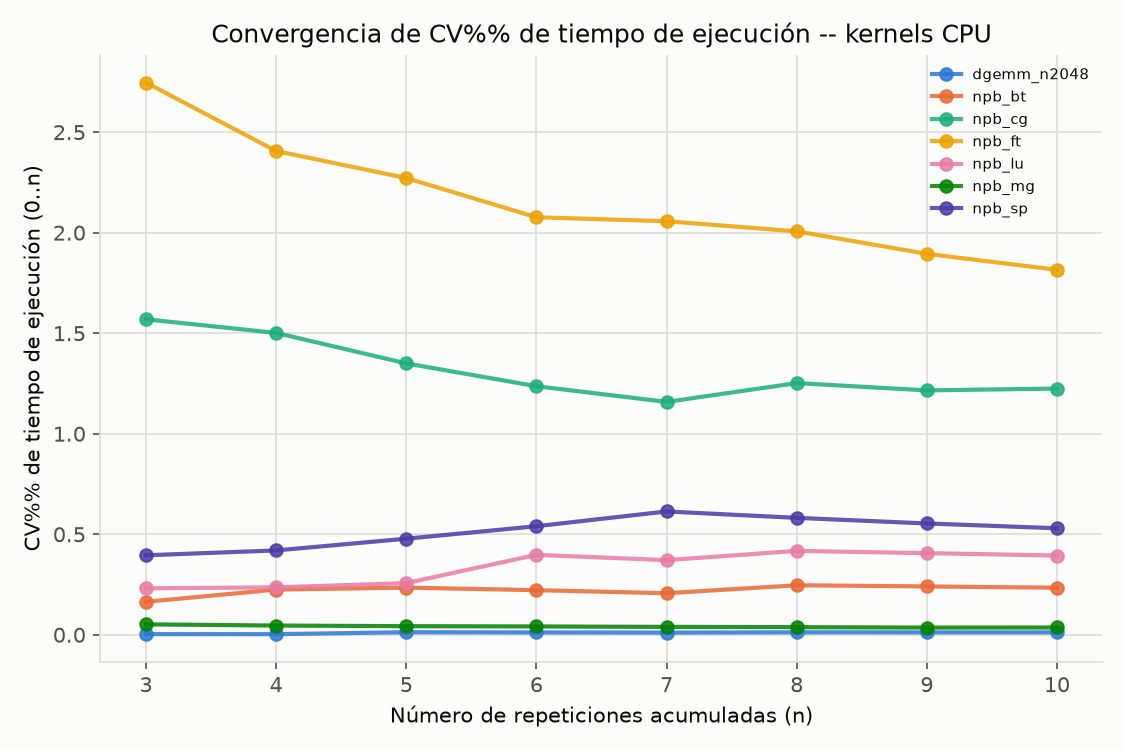
\includegraphics[width=0.85\textwidth]{../plots/repetitions/cv_convergence_vs_repetitions_cpu.png}
\caption{Convergencia de CV\% de tiempo de ejecución vs. repeticiones
acumuladas, kernels CPU.}
\label{fig:rep-cpu}
\end{figure}

\begin{figure}[H]
\centering
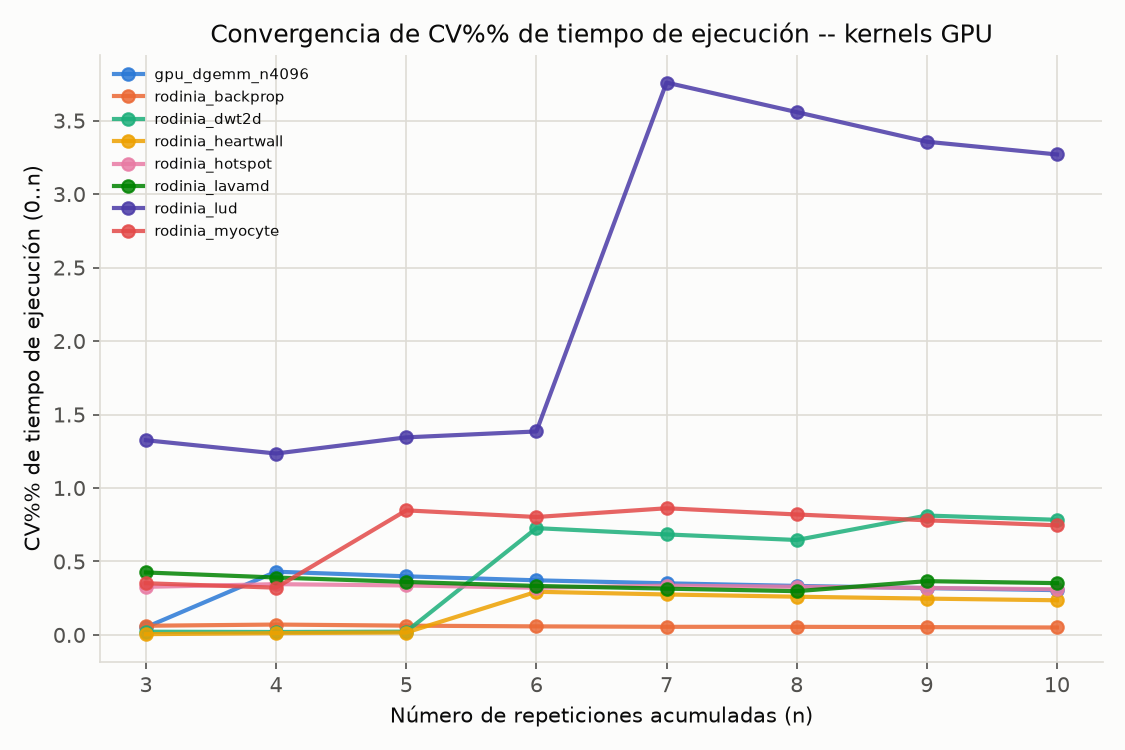
\includegraphics[width=0.85\textwidth]{../plots/repetitions/cv_convergence_vs_repetitions_gpu.png}
\caption{Convergencia de CV\% de tiempo de ejecución vs. repeticiones
acumuladas, kernels GPU. El salto de \texttt{rodinia\_lud} en $n=7$ es una
repetición atípica real, no un artefacto de graficación.}
\label{fig:rep-gpu}
\end{figure}

\subsection{El CV\% de "las primeras tres" depende del orden -- reanálisis combinatorio}

El CV\% a $n=3$ reportado arriba usa siempre las primeras tres de las diez
repeticiones, en el orden fijo en que se ejecutaron. Eso es exactamente el
grupo de tres que una campaña real con \texttt{repetitions\_per\_combination=3}
habría medido -- pero no dice nada sobre qué tan representativo es ese
grupo particular frente a cualquier otro trío posible. Para responder eso,
se recalculó el CV\% de tiempo de ejecución sobre las
$\binom{10}{3}=120$ combinaciones posibles de tres repeticiones de cada
kernel (mismos datos, sin cómputo nuevo), y se compara la muestra de orden
fijo contra la distribución completa (Tabla~\ref{tab:combinatoric-cv3}).

\textbf{Nota metodológica sobre el estimador}: todos los CV\% de esta
sección (y del resto del informe) se calculan con desviación estándar
\emph{poblacional} (\texttt{statistics.pstdev}, denominador $n$), no
muestral (denominador $n-1$). Para $n=3$, la desviación muestral es un
factor $\sqrt{3/2}\approx 1{,}22$ mayor que la poblacional -- es decir,
todos los CV\% a $n=3$ reportados aquí subestiman en $\sim$22\,\% lo que
un cálculo con el estimador insesgado habitual (muestral) reportaría. Esto
no cambia ninguna conclusión cualitativa (qué kernel es más o menos
estable, dónde está la anomalía de \texttt{rodinia\_lud}), pero sí debe
declararse: el margen real de cualquier comparación contra un umbral de
CV\% en este informe es algo más estrecho de lo que las cifras crudas
sugieren.

\begin{table}[H]
\centering
\caption{CV\% de tiempo de ejecución con 3 repeticiones: valor de orden fijo vs. distribución sobre las 120 combinaciones posibles (casos más informativos).}
\label{tab:combinatoric-cv3}
\small
\begin{tabular}{@{}lrrrrr@{}}
\toprule
\textbf{Kernel} & \textbf{orden fijo} & \textbf{mediana} & \textbf{p95} & \textbf{máx} & \textbf{CV\% con n=10} \\
\midrule
\texttt{rodinia\_lud}    & 1{,}32\,\% & 1{,}35\,\% & 5{,}27\,\% & 5{,}49\,\% & 3{,}27\,\% \\
\texttt{npb\_ft}         & 2{,}75\,\% & 1{,}10\,\% & 2{,}51\,\% & 2{,}75\,\% & 1{,}81\,\% \\
\texttt{rodinia\_dwt2d}  & 0{,}02\,\% & 0{,}91\,\% & 0{,}93\,\% & 0{,}93\,\% & 0{,}78\,\% \\
\texttt{rodinia\_myocyte}& 0{,}35\,\% & 0{,}36\,\% & 1{,}21\,\% & 1{,}25\,\% & 0{,}75\,\% \\
\texttt{npb\_cg}         & 1{,}57\,\% & 0{,}91\,\% & 1{,}78\,\% & 1{,}92\,\% & 1{,}23\,\% \\
\bottomrule
\end{tabular}
\end{table}

Dos patrones reales aparecen, y son distintos entre sí:

\begin{itemize}
  \item \textbf{\texttt{rodinia\_lud}}: el trío de orden fijo (1{,}32\,\%) y
    la mediana de los 120 tríos (1{,}35\,\%) coinciden -- la mayoría de los
    tríos posibles \emph{no} incluyen la repetición atípica (rep07). Pero
    el percentil 95 (5{,}27\,\%) y el máximo (5{,}49\,\%) muestran que un
    trío con mala suerte sí la detectaría con un CV\% muy por encima del
    umbral típico de calibración (D03=40\,\% es otro parámetro, no
    comparable directamente, pero un 5\,\% ya es una señal visible en
    cualquier chequeo de estabilidad con umbral de un dígito). Es decir:
    tres repeticiones \emph{pueden} detectar esta anomalía, pero depende
    del azar de cuáles tres se corran -- no es una garantía ni una omisión
    sistemática.
  \item \textbf{\texttt{rodinia\_dwt2d}}: el caso inverso. El trío de orden
    fijo (0{,}02\,\%) es un caso particularmente favorable -- la mediana
    real (0{,}91\,\%) y el CV\% a $n=10$ (0{,}78\,\%) son casi 40 veces
    más altos. Aquí el riesgo no es una anomalía puntual sino que la
    muestra de tres repeticiones normalmente vista subestima la
    variabilidad real del kernel por casi dos órdenes de magnitud respecto
    al trío que efectivamente corrió.
\end{itemize}

\textbf{Conclusión (reformulada tras el reanálisis combinatorio)}: tres
repeticiones constituyen un \textbf{mínimo operativo razonable para la
adquisición de Fase 1} en los kernels alejados de la frontera de
clasificación Roofline, no una demostración de que tres repeticiones
estimen con precisión la variabilidad real de cada kernel ni que
garanticen detectar eventos infrecuentes -- ambas cosas dependen de qué
trío particular se ejecute, como muestra la dispersión completa de
\texttt{rodinia\_lud} y \texttt{rodinia\_dwt2d}. Esta limitación es más
seria para la evaluación de energía y EDP de Fase 4 que para la
adquisición de Fase 1: este barrido caracterizó variabilidad de
\emph{tiempo de ejecución}, no variabilidad energética, y no hay evidencia
todavía de que tres repeticiones sean suficientes para estimar el EDP con
la misma confianza. Para Fase 4 conviene usar más repeticiones o un
criterio adaptativo basado en el ancho del intervalo de confianza
observado, en vez de heredar sin más el mínimo de Fase 1.

\subsection{Suficiencia de \texttt{target\_windows\_per\_repetition}}

Usando las mismas 150 corridas, la Tabla~\ref{tab:target-windows} reporta,
para cada kernel, el mínimo de ventanas útiles logradas en cualquiera de
las diez repeticiones (\texttt{windows\_achieved\_min}) frente al objetivo
configurado (50 para CPU, 5 para GPU). En los 15 kernels del catálogo, el
mínimo observado supera el objetivo por al menos un orden de magnitud
(\texttt{npb\_mg}, el caso más ajustado del lado CPU, con 629 ventanas
mínimas frente a un objetivo de 50; \texttt{rodinia\_backprop}, el más
ajustado del lado GPU, con 140 frente a un objetivo de 5).

\begin{table}[H]
\centering
\caption{Ventanas útiles logradas (media y mínimo sobre 10 repeticiones) vs. objetivo configurado.}
\label{tab:target-windows}
\small
\begin{tabular}{@{}lrrr@{}}
\toprule
\textbf{Kernel} & \textbf{Objetivo} & \textbf{Media} & \textbf{Mínimo} \\
\midrule
\texttt{dgemm\_n2048} & 50 & 2464{,}7 & 2457 \\
\texttt{npb\_bt} & 50 & 24920{,}5 & 24828 \\
\texttt{npb\_cg} & 50 & 6692{,}7 & 6605 \\
\texttt{npb\_ft} & 50 & 3718{,}4 & 3649 \\
\texttt{npb\_lu} & 50 & 16347{,}1 & 16212 \\
\texttt{npb\_mg} & 50 & 637{,}1 & 629 \\
\texttt{npb\_sp} & 50 & 16758{,}7 & 16601 \\
\midrule
\texttt{gpu\_dgemm\_n4096} & 5 & 798{,}2 & 750 \\
\texttt{rodinia\_backprop} & 5 & 148{,}0 & 140 \\
\texttt{rodinia\_dwt2d} & 5 & 375{,}2 & 366 \\
\texttt{rodinia\_heartwall} & 5 & 1064{,}3 & 1058 \\
\texttt{rodinia\_hotspot} & 5 & 1231{,}6 & 1165 \\
\texttt{rodinia\_lavamd} & 5 & 980{,}7 & 922 \\
\texttt{rodinia\_lud} & 5 & 1564{,}2 & 1413 \\
\texttt{rodinia\_myocyte} & 5 & 1152{,}4 & 1113 \\
\bottomrule
\end{tabular}
\end{table}

\textbf{Conclusión (con el alcance correcto del chequeo)}: los datos
demuestran con claridad que \texttt{target\_windows\_per\_repetition}
\textbf{no condiciona el catálogo actual} -- en ningún caso observado
(150 corridas) estuvo cerca de ser la restricción activa, y el margen es
tan amplio (10--500$\times$ el objetivo contando lecturas crudas) que el
valor exacto configurado (50 o 5) no cambia qué corridas se aceptan hoy.
Eso es una afirmación distinta, y más débil, de decir que 50 o 5 son un
\emph{mínimo estadísticamente suficiente}: las ventanas contiguas de un
mismo kernel están correlacionadas entre sí (no son extracciones
independientes de una distribución), y para los kernels GPU, la
Sección~\ref{sec:gpu-interval-ns} muestra que varias "ventanas" NVML
consecutivas pueden compartir el mismo valor de sensor subyacente -- 5
lecturas GPU no equivalen necesariamente a 5 observaciones físicas
distintas. \texttt{target\_windows\_per\_repetition} debe entenderse,
entonces, como un \textbf{guardarraíl de duración mínima de la corrida}
(evita aceptar un kernel que termina casi de inmediato, sin tiempo
suficiente para que el detector de calentamiento y el resto del pipeline
operen con sentido) y no como una prueba de suficiencia estadística de la
muestra resultante. En la práctica, para el catálogo actual, ese
guardarraíl nunca es la restricción activa -- los seis casos ya
documentados con evidencia negativa de calentamiento (ARC-86) son
precisamente ejemplos de kernels cerca del límite en duración total,
aunque no en conteo de ventanas -- pero esto no debe leerse como una
validación de que el dataset resultante tiene suficiencia estadística
para ningún uso posterior (por ejemplo, entrenamiento de un modelo en
Fase 2): esa es una pregunta distinta, que requiere su propio análisis
de partición por corrida/carga, balance de clases y evaluación fuera de
muestra.

